\documentclass[dvipdfmx]{jsarticle}

\usepackage{geometry}                                                              %余白調整.オプション追加してお好みで変えることも出来る.
%プログラムソースコード記述に関する設定

\usepackage{listings,jlisting} %日本語のコメントアウトをする場合jlistingが必要
%ここからソースコードの表示に関する設定
\lstset{
  basicstyle={\ttfamily},
  identifierstyle={\small},
  commentstyle={\smallitshape},
    keywordstyle={\small\bfseries},
  ndkeywordstyle={\small},
  stringstyle={\small\ttfamily},
  frame={tb},
  breaklines=true,
  columns=[l]{fullflexible},
  numbers=left,
  xrightmargin=0zw,
  xleftmargin=3zw,
  numberstyle={\scriptsize},
  stepnumber=1,
  numbersep=1zw,
  lineskip=-0.5ex
}
%ここまでソースコードの表示に関する設定


%テキストの表示領域の調節
\setlength{\textwidth}{\paperwidth}
\addtolength{\textwidth}{-40truemm}
\setlength{\textheight}{\paperheight}
\addtolength{\textheight}{-45truemm}

%余白の調節
\setlength{\topmargin}{-10.4truemm}
\setlength{\evensidemargin}{-5.4truemm}
\setlength{\oddsidemargin}{-5.4truemm}
\setlength{\headheight}{17pt}
\setlength{\headsep}{10mm}
\addtolength{\headsep}{-17pt}
\setlength{\footskip}{5mm}

%右上にページ番号
\usepackage{fancyhdr}
\pagestyle{fancy}
\lhead{}
\rhead{}
\rhead{\thepage{}}
\cfoot{}
\renewcommand{\headrulewidth}{0pt}

\usepackage{here}

\usepackage{tabularx}

\usepackage{siunitx}                                                               %単位を書くのに使いましょう
\usepackage{url}                                                                   %URLを書く時に使いましょう

\usepackage[dvipdfmx]{graphicx}
\usepackage{tikz}                                                                  %てぃくす.図を描くのに便利.ググったら使い方は出て来る.英語に自信があるならここのマニュアルhttp://ftp.yz.yamagata-u.ac.jp/pub/CTAN/graphics/pgf/base/doc/pgfmanual.pdf
\usetikzlibrary{arrows,decorations.pathmorphing,backgrounds,positioning,fit,petri} %TikZに必要なものに応じて変えてね.実際にはここではこれ全部は使って無い.上のマニュアルの3 Tutorial: A Petri-Net for HagenのSetting up the Environment in LATEXに従った.

\begin{document}
    \section{目的}
  CPUのシミュレーションプログラム作成を通しCPUの動作を理解する.
    \section{実習}
      \subsection{実習7:一方向の連結リスト}

      \begin{table}[h]
        \centering
        \caption{一方向連結リストソースコード}
        \label{tab:list}
        \begin{tabular}{c|cc|cc|ccc}
          \hline \hline
          Address & obj & code & source  & code &  &  &  \\ \hline
          00 & 67 & 00 & START: & LD & mem(IX+00H), & ACC & mem(IX+00H)-$>$AC\\
          02 & 6f & 01 &  & LD & mem(IX+00H), & IX & mem(IX+00H)-$>$IX \\
          04 & fa & 00 &  & CMP & IX, & 0 & IX-00H \\
          06 & 39 & 11 &  & BZ & END: &  & ZF=1? \\
          08 & f5 & ff &  & CMP & ACC, & mem[1ffH] & ACC-mem[1ffH] \\
          0a & 3a & 0e &  & BN & P1: &  & NF=1? \\
          0c & 75 & ff &  & ST & ACC, & mem[1ffH] & ACC-$>$mem[1ffH] \\
          0e & 62 & 00 & P1: & LD & 00H & ACC & 00H-$>$ACC \\
          10 & 0b &  &  & JR & START: &  &  \\
          11 & 0f &  & END: &  &  &  &  \\ \hline

        \end{tabular}
      \end{table}

\begin{figure}[h]
  \centering
  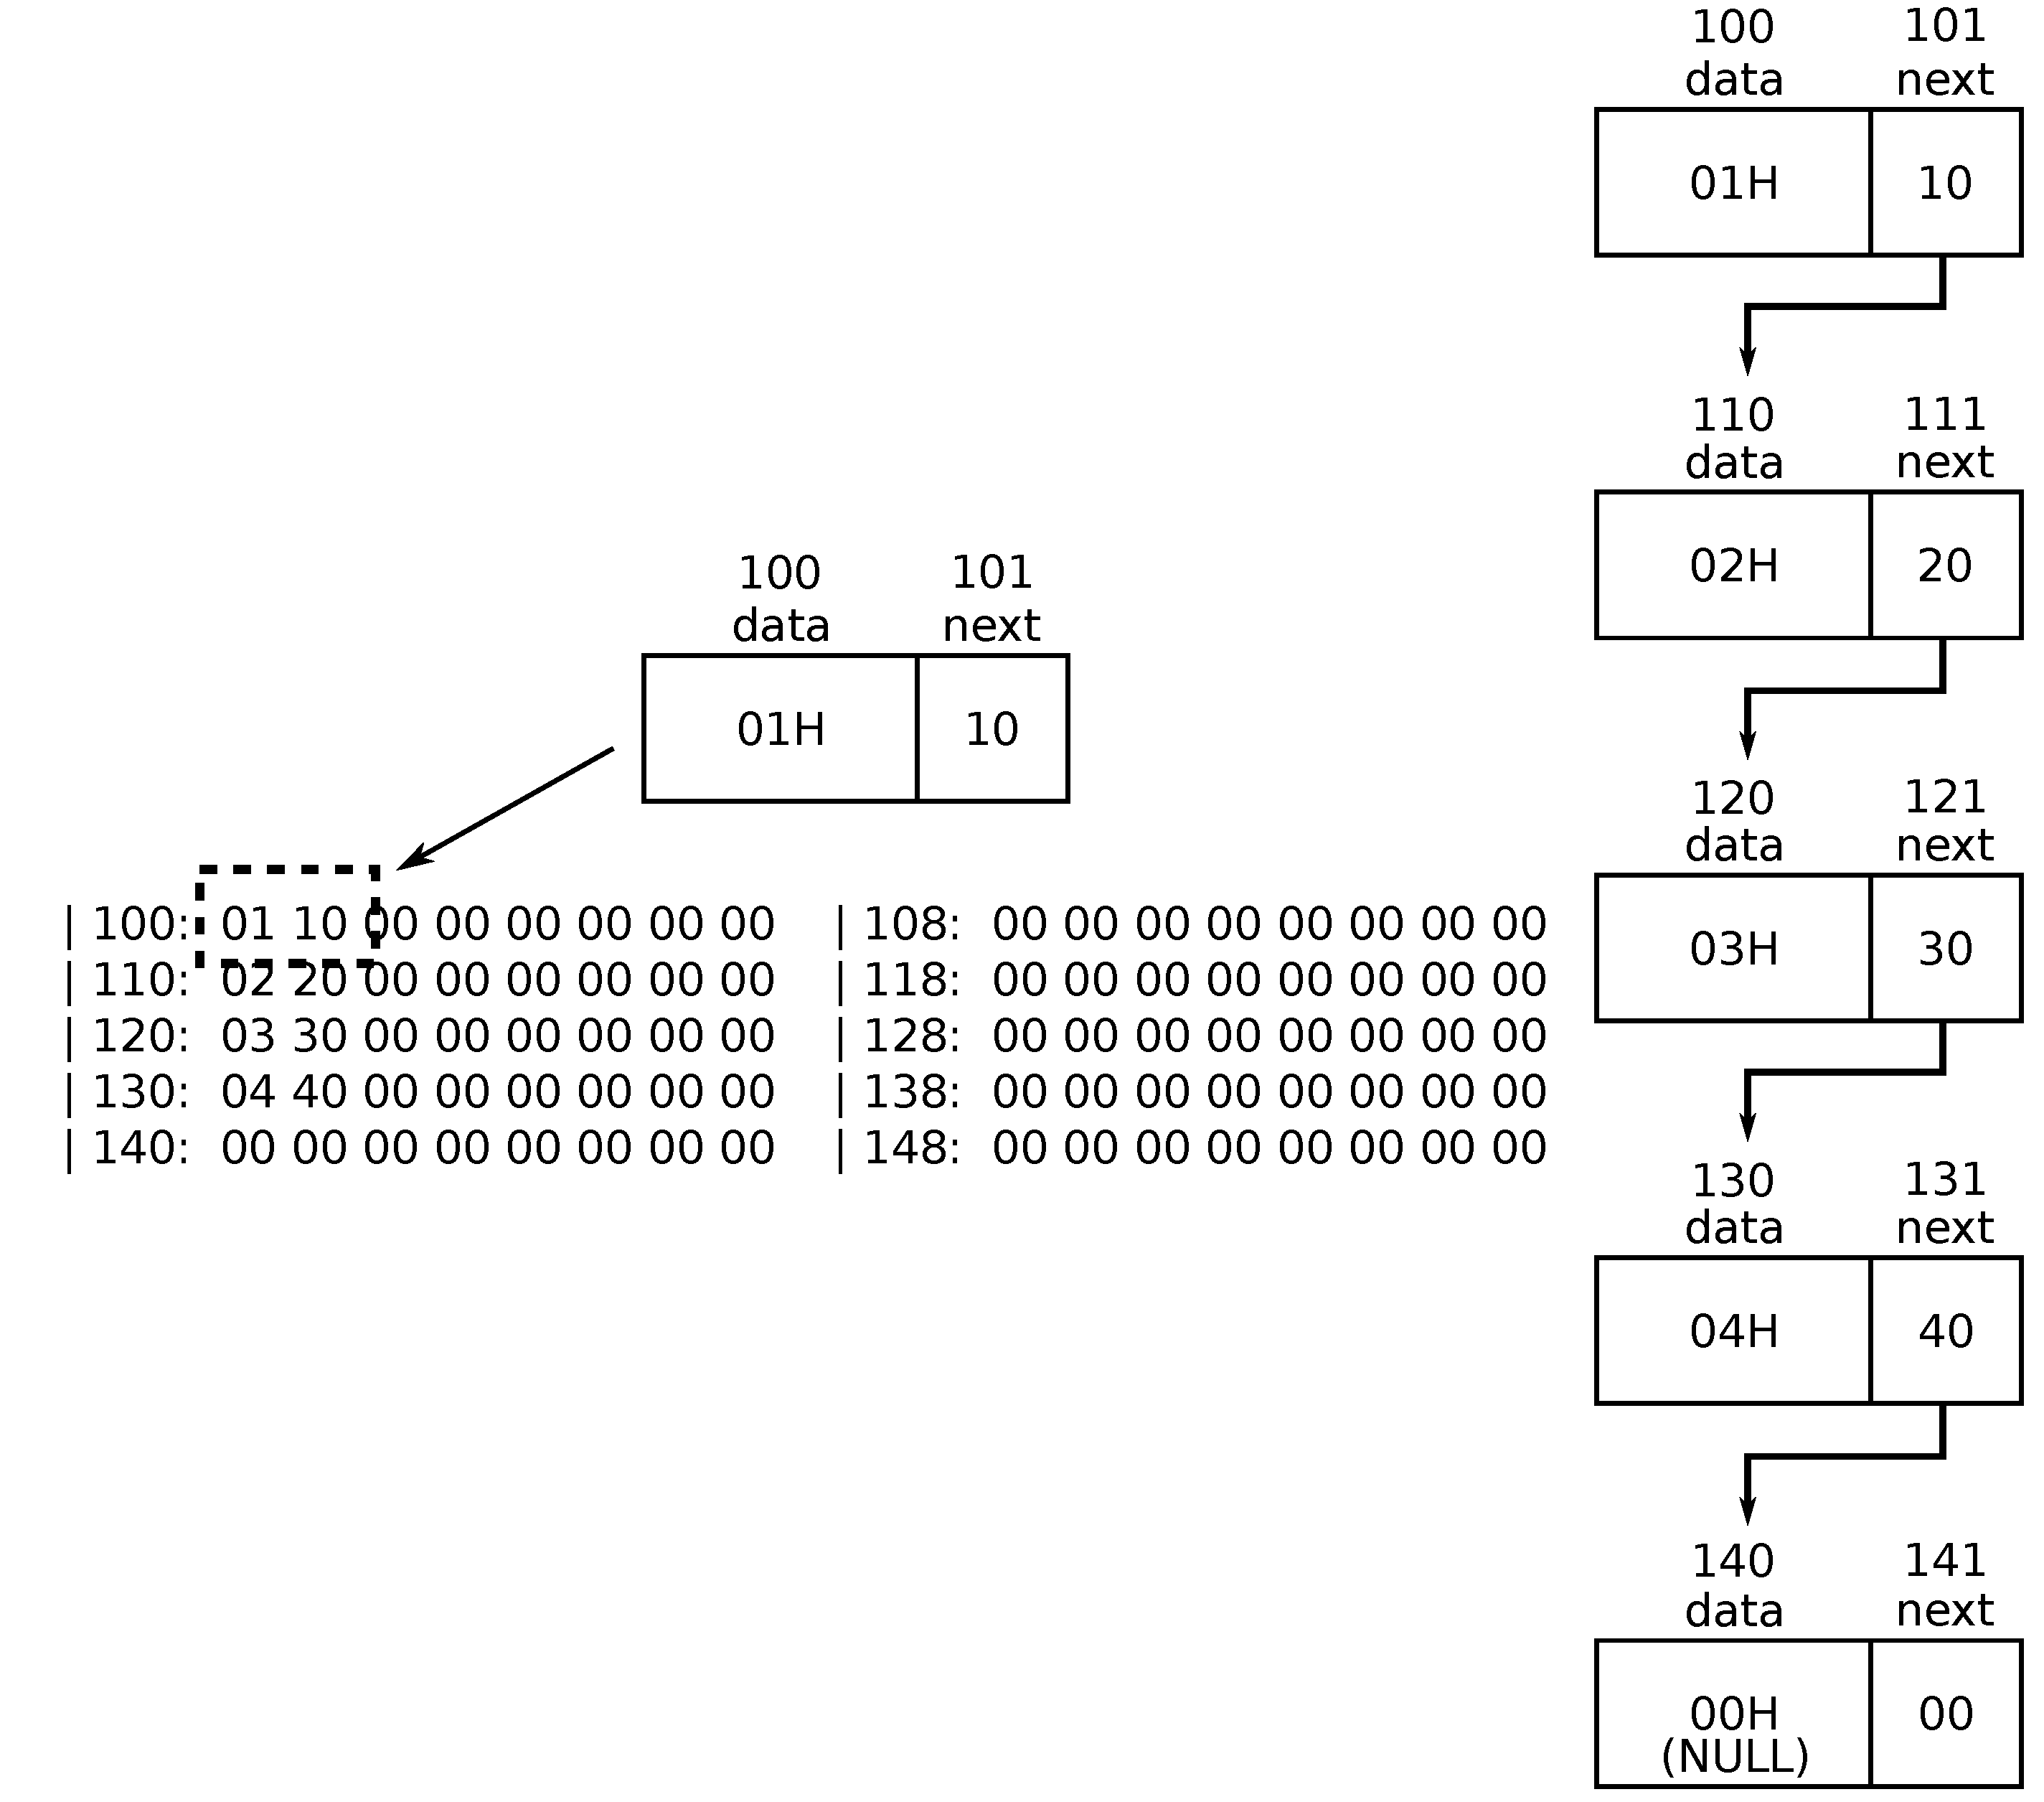
\includegraphics[width=8cm]{7_list.pdf}
  \caption{データ構造:リスト}
  \label{fig:7_list}
\end{figure}


\begin{figure}[h]
  \centering
  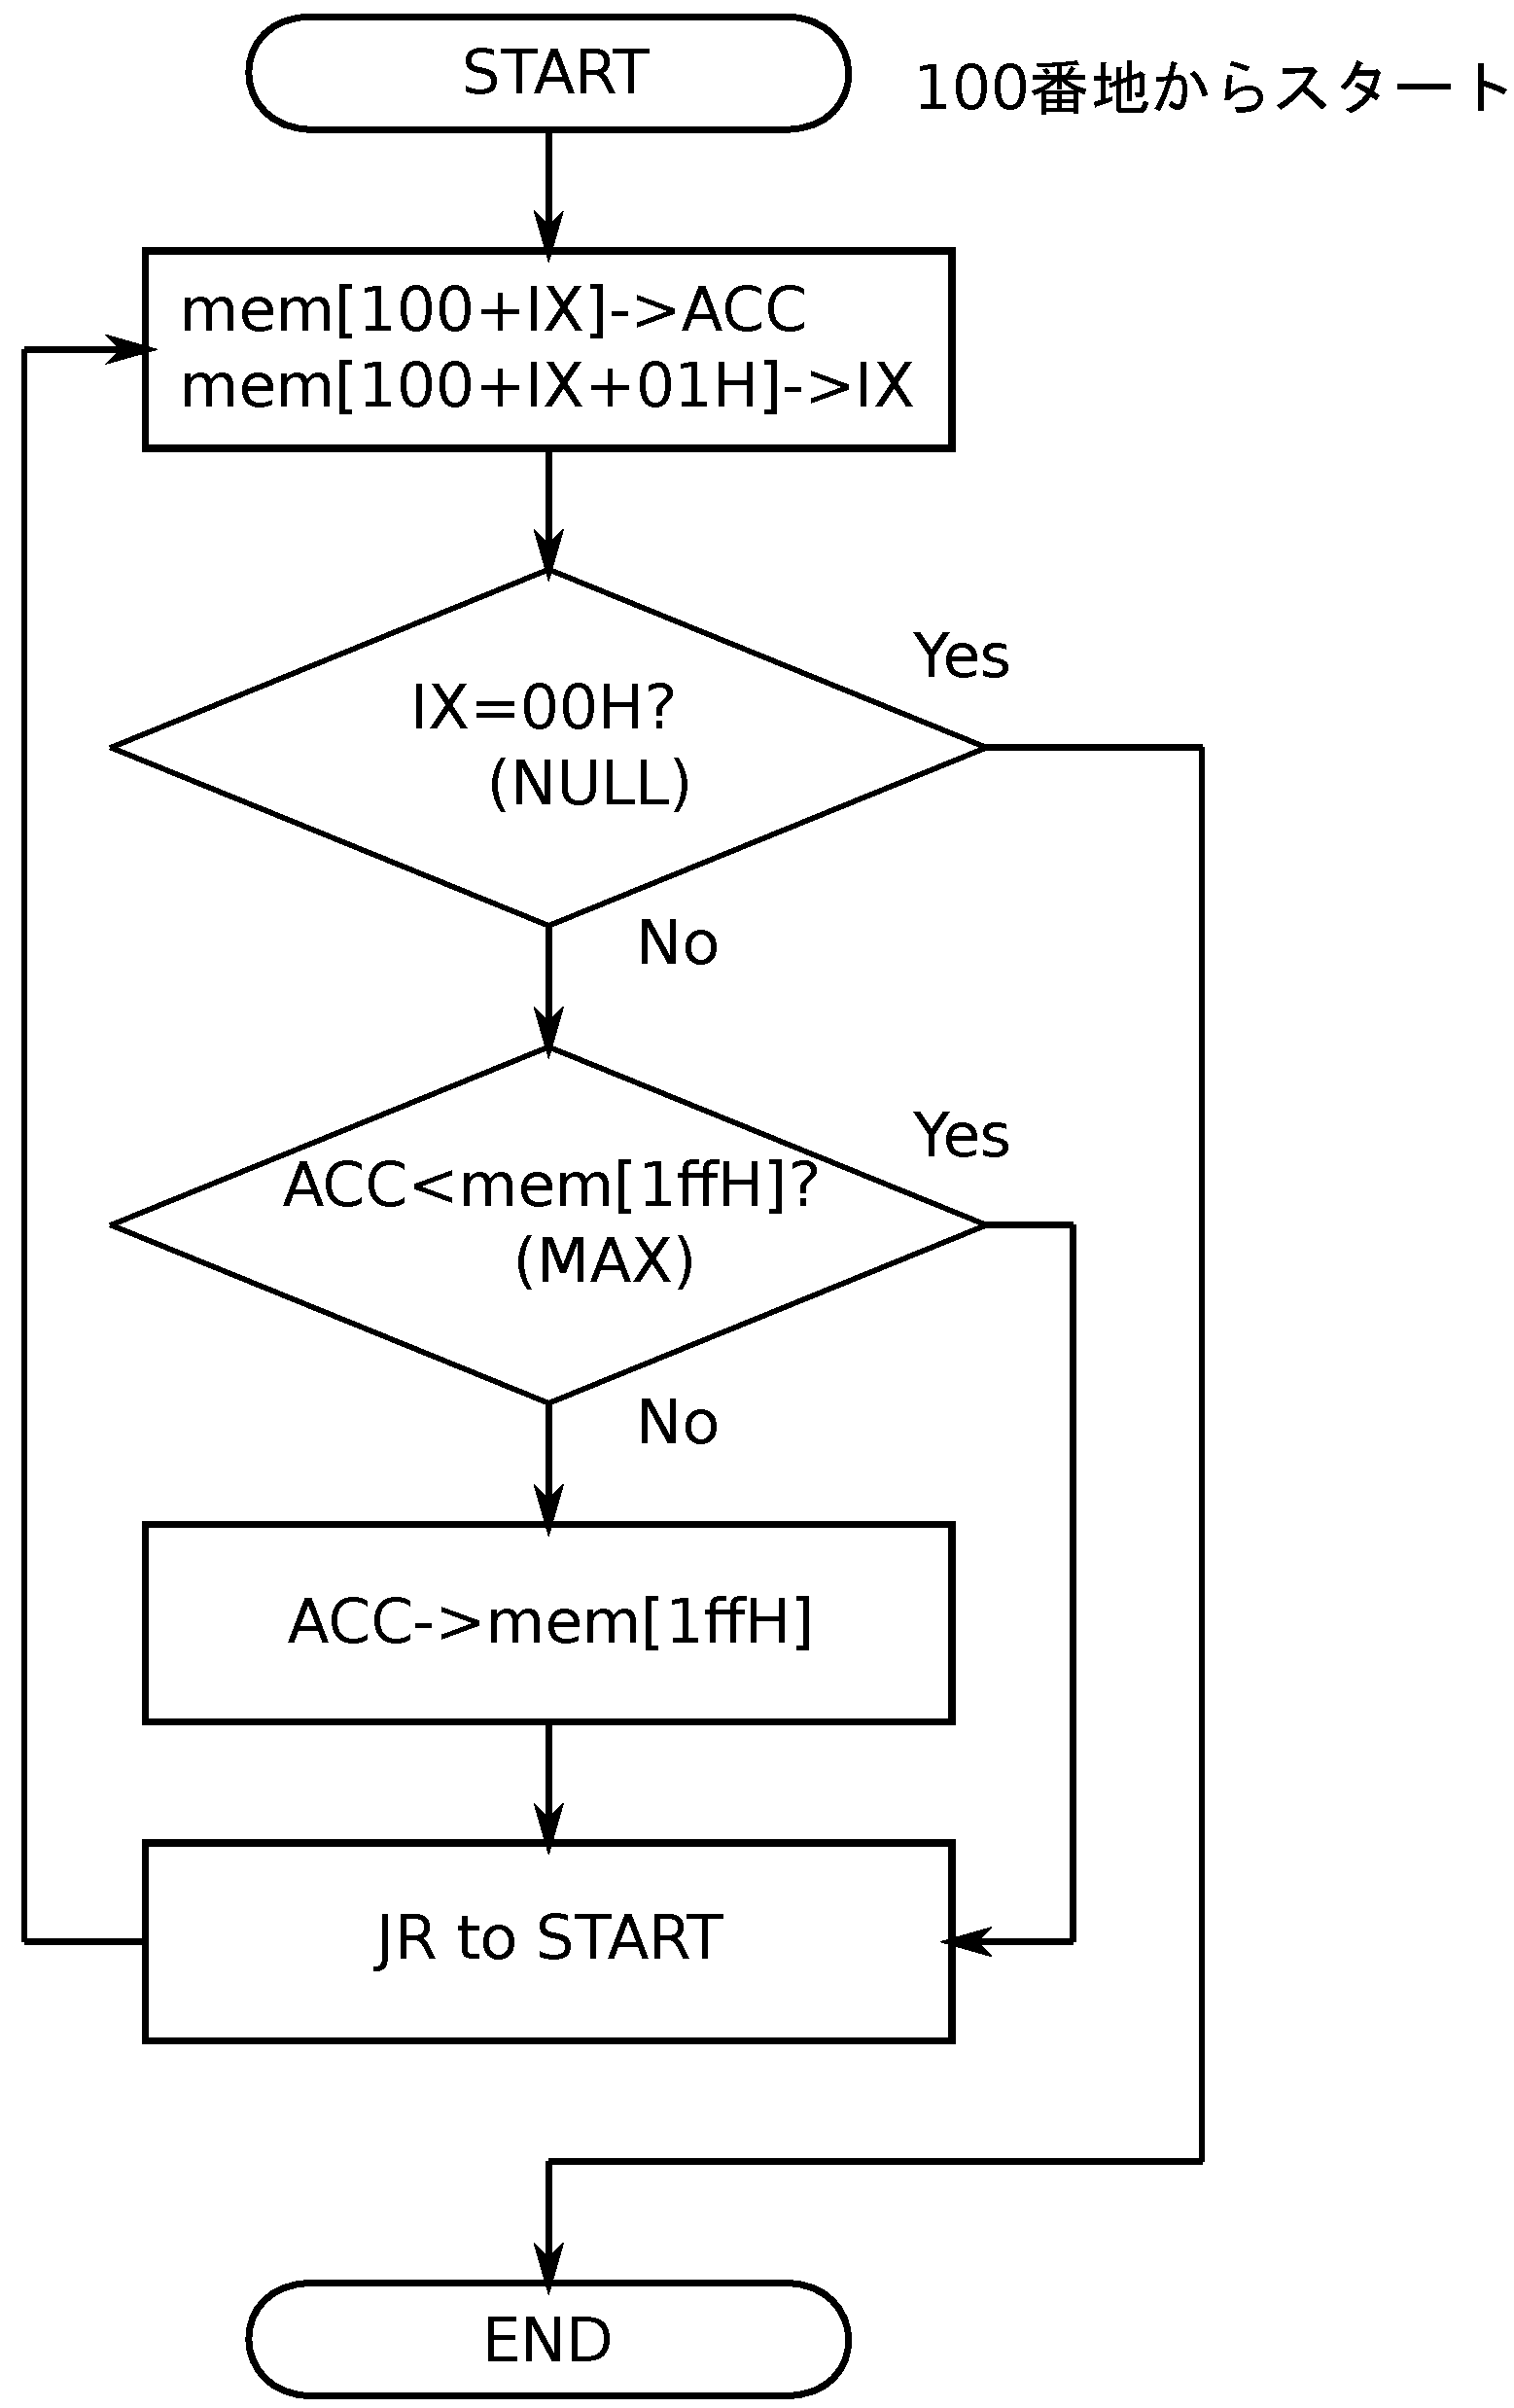
\includegraphics[width=8cm]{7_list_flow.pdf}
  \caption{実習7:一方向連結リストフローチャート}
  \label{fig:7_list_flow}
\end{figure}


表\ref{tab:list}に一方向連結リストプログラムソースコードを示す.mem[100]へdata,mem[101]へnextとして考え.スタート位置はmem[100H]をスタート位置とした.\\
dataが格納されているメモリの隣にアドレスを格納しており、アドレスをIXへ格納して次のdataを参照するようになっている.dataはACCへ格納後,これまで参照した最大値が格納されているメモリ(mem[1ffH])と比較しACCの方が大きければ入れ替え動作を行う.\\
NULLは00Hとしnextで参照した先が00の場合終了する.
表\ref{tab:list}に示すのデータ構造を以下に示す.
\newpage
以下に結果を示す.
結果よりmem[1ffH]へ最大値の04Hが格納され終了しているためプログラムは正しく実行されたと確認できる.
      \begin{verbatim}
CPU0,PC=0x0> r 7_list.CPU0,PC=0x0> m 0
    | 000:  67 00 6f 01 fa 00 39 11    | 008:  f5 ff 3a 0e 75 ff 62 00
CPU0,PC=0x0> m 10
    | 010:  0b 0f 00 00 00 00 00 00    | 018:  00 00 00 00 00 00 00 00
CPU0,PC=0x0> m 100
    | 100:  01 10 00 00 00 00 00 00    | 108:  00 00 00 00 00 00 00 00
CPU0,PC=0x0> m 110
    | 110:  02 20 00 00 00 00 00 00    | 118:  00 00 00 00 00 00 00 00
CPU0,PC=0x0> m 120
    | 120:  03 30 00 00 00 00 00 00    | 128:  00 00 00 00 00 00 00 00
CPU0,PC=0x0> m 130
    | 130:  04 40 00 00 00 00 00 00    | 138:  00 00 00 00 00 00 00 00
CPU0,PC=0x0> m 140
    | 140:  00 00 00 00 00 00 00 00    | 148:  00 00 00 00 00 00 00 00
CPU0,PC=0x0> m 1f0
    | 1f0:  00 00 00 00 00 00 00 00    | 1f8:  00 00 00 00 00 00 00 00
CPU0,PC=0x0>c 10
CPU0,PC=0x10> m 1f0
    | 1f0:  00 00 00 00 00 00 00 00    | 1f8:  00 00 00 00 00 00 00 01
CPU0,PC=0x10> d
	acc=0x00(0,0)    ix=0x10(16,16)   cf=0 vf=0 nf=0 zf=0
	ibuf=0:0x00(0,0)    obuf=0:0x00(0,0)
CPU0,PC=0x10> i
CPU0,PC=0x0> c 10
CPU0,PC=0x10> m 1f0
    | 1f0:  00 00 00 00 00 00 00 00    | 1f8:  00 00 00 00 00 00 00 02
CPU0,PC=0x10> d
	acc=0x00(0,0)    ix=0x20(32,32)   cf=0 vf=0 nf=0 zf=0
	ibuf=0:0x00(0,0)    obuf=0:0x00(0,0)
CPU0,PC=0x10> i
CPU0,PC=0x0> c 10
CPU0,PC=0x10> m 1f0
    | 1f0:  00 00 00 00 00 00 00 00    | 1f8:  00 00 00 00 00 00 00 03
CPU0,PC=0x10> d
	acc=0x00(0,0)    ix=0x30(48,48)   cf=0 vf=0 nf=0 zf=0
	ibuf=0:0x00(0,0)    obuf=0:0x00(0,0)
CPU0,PC=0x10> i
CPU0,PC=0x0> c 10
CPU0,PC=0x10> m 1f0
    | 1f0:  00 00 00 00 00 00 00 00    | 1f8:  00 00 00 00 00 00 00 04
CPU0,PC=0x10> d
	acc=0x00(0,0)    ix=0x40(64,64)   cf=0 vf=0 nf=0 zf=0
	ibuf=0:0x00(0,0)    obuf=0:0x00(0,0)
CPU0,PC=0x10> i
CPU0,PC=0x0> c 10
Program Halted.
CPU0,PC=0x12> m 1f0
| 1f0:  00 00 00 00 00 00 00 00    | 1f8:  00 00 00 00 00 00 00 04
CPU0,PC=0x12> d
	acc=0x00(0,0)    ix=0x00(0,0)   cf=0 vf=0 nf=0 zf=1
	ibuf=0:0x00(0,0)    obuf=0:0x00(0,0)
CPU0,PC=0x12>

      \end{verbatim}


\newpage
      \subsection{実習8:データ通信プログラム}

      \begin{table}[h]
        \centering
        \caption{データ通信プログラム送信側}
        \label{tab:out}
        \begin{tabular}{c|cc|cc|ccc}
          \hline \hline

          Address & obj & code & source  & code &  &  &  \\ \hline
          00 & 62 & 03 & START: & LD & 03H(要素数), & ACC & 03H-$>$ACC \\
          02 & 10 &  &  & OUT &  &  & ACC-$>$OBUF \\
          03 & 3c & 03 & WAIT: & BNO & WAIT: &  & OBUF\_FLG\_IN=1? \\
          05 & 6a & 00 &  & LD & 01H, & IX & 01H-$>$IX \\
          07 & 62 & 01 &  & LD & 01H, & ACC & 01H-$>$ACC \\
          09 & 10 &  &  & OUT &  &  & ACC-$>$OBUF \\
          0a & 3c & 0a & WAIT2: & BNO & WAIT2: &  & OBUF\_FLG\_IN=1? \\
          0c & ba & 01 &  & ADD & IX, & 01H & IX+01H-$>$IX \\
          0e & b2 & 01 &  & ADD & ACC, & 01H & ACC+01H-$>$ACC \\
          10 & fa & 03 &  & CMP & IX, & 03H & IX-03H \\
          12 & 31 & 09 &  & BNZ & WAIT2: &  & (NF v ZF) = 1 \\
          14 & 0f &  &  & HLT &  &  &  \\ \hline

        \end{tabular}
      \end{table}

      \begin{table}[h]
        \centering
        \caption{データ通信プログラム受信側}
        \label{tab:in}
        \begin{tabular}{c|cc|cc|ccc}
          \hline \hline

          Address & obj & code & source  & code &  &  &  \\ \hline
          00 & 34 & 00 & WAIT: & BNI & WAIT: &  & IBUF_FLG_IN=0? \\
          02 & 1f &  &  & IN &  &  & IBUF-$>$ACC \\
          03 & 75 & c0 &  & ST & ACC, & mem[1C0H] & ACC-$>$mem[1c0H] \\
          05 & 6a & 00 &  & LD & 00H & IX, & 00H-$>$IX \\
          07 & 34 & 07 & LOOP: & BNI & LOOP: &  & IBUF\_FLG\_IN=0? \\
          09 & 1f &  &  & IN &  &  & IBUF-$>$ACC \\
          0a & b5 & 03 &  & ADD & ACC, & mem[103H] & ACC+mem[103H]-$>$ACC \\
          0c & 75 & 03 &  & ST & ACC, & mem[103H] & ACC+mem[103H]-$>$ACC \\
          0e & ba & 01 &  & ADD & IX, & 01H & IX+01H-$>$IX \\
          10 & fd & c0 &  & CMP & IX, & mem[1C0H] & IX+mem[1c0H] \\
          12 & 31 & 07 &  & BNZ & LOOP: &  & ZF=0? \\
          14 & 0f &  &  & HLT &  &  &  \\ \hline

        \end{tabular}
      \end{table}

表\ref{tab:out},\ref{tab:in}にデータ通信プログラムソースコードを示す.表\ref{tab:out}では要素数を即値を用いて通信相手の受け取りが確認できるまでWAITでループ待機する.

\begin{figure}[h]
  \centering
  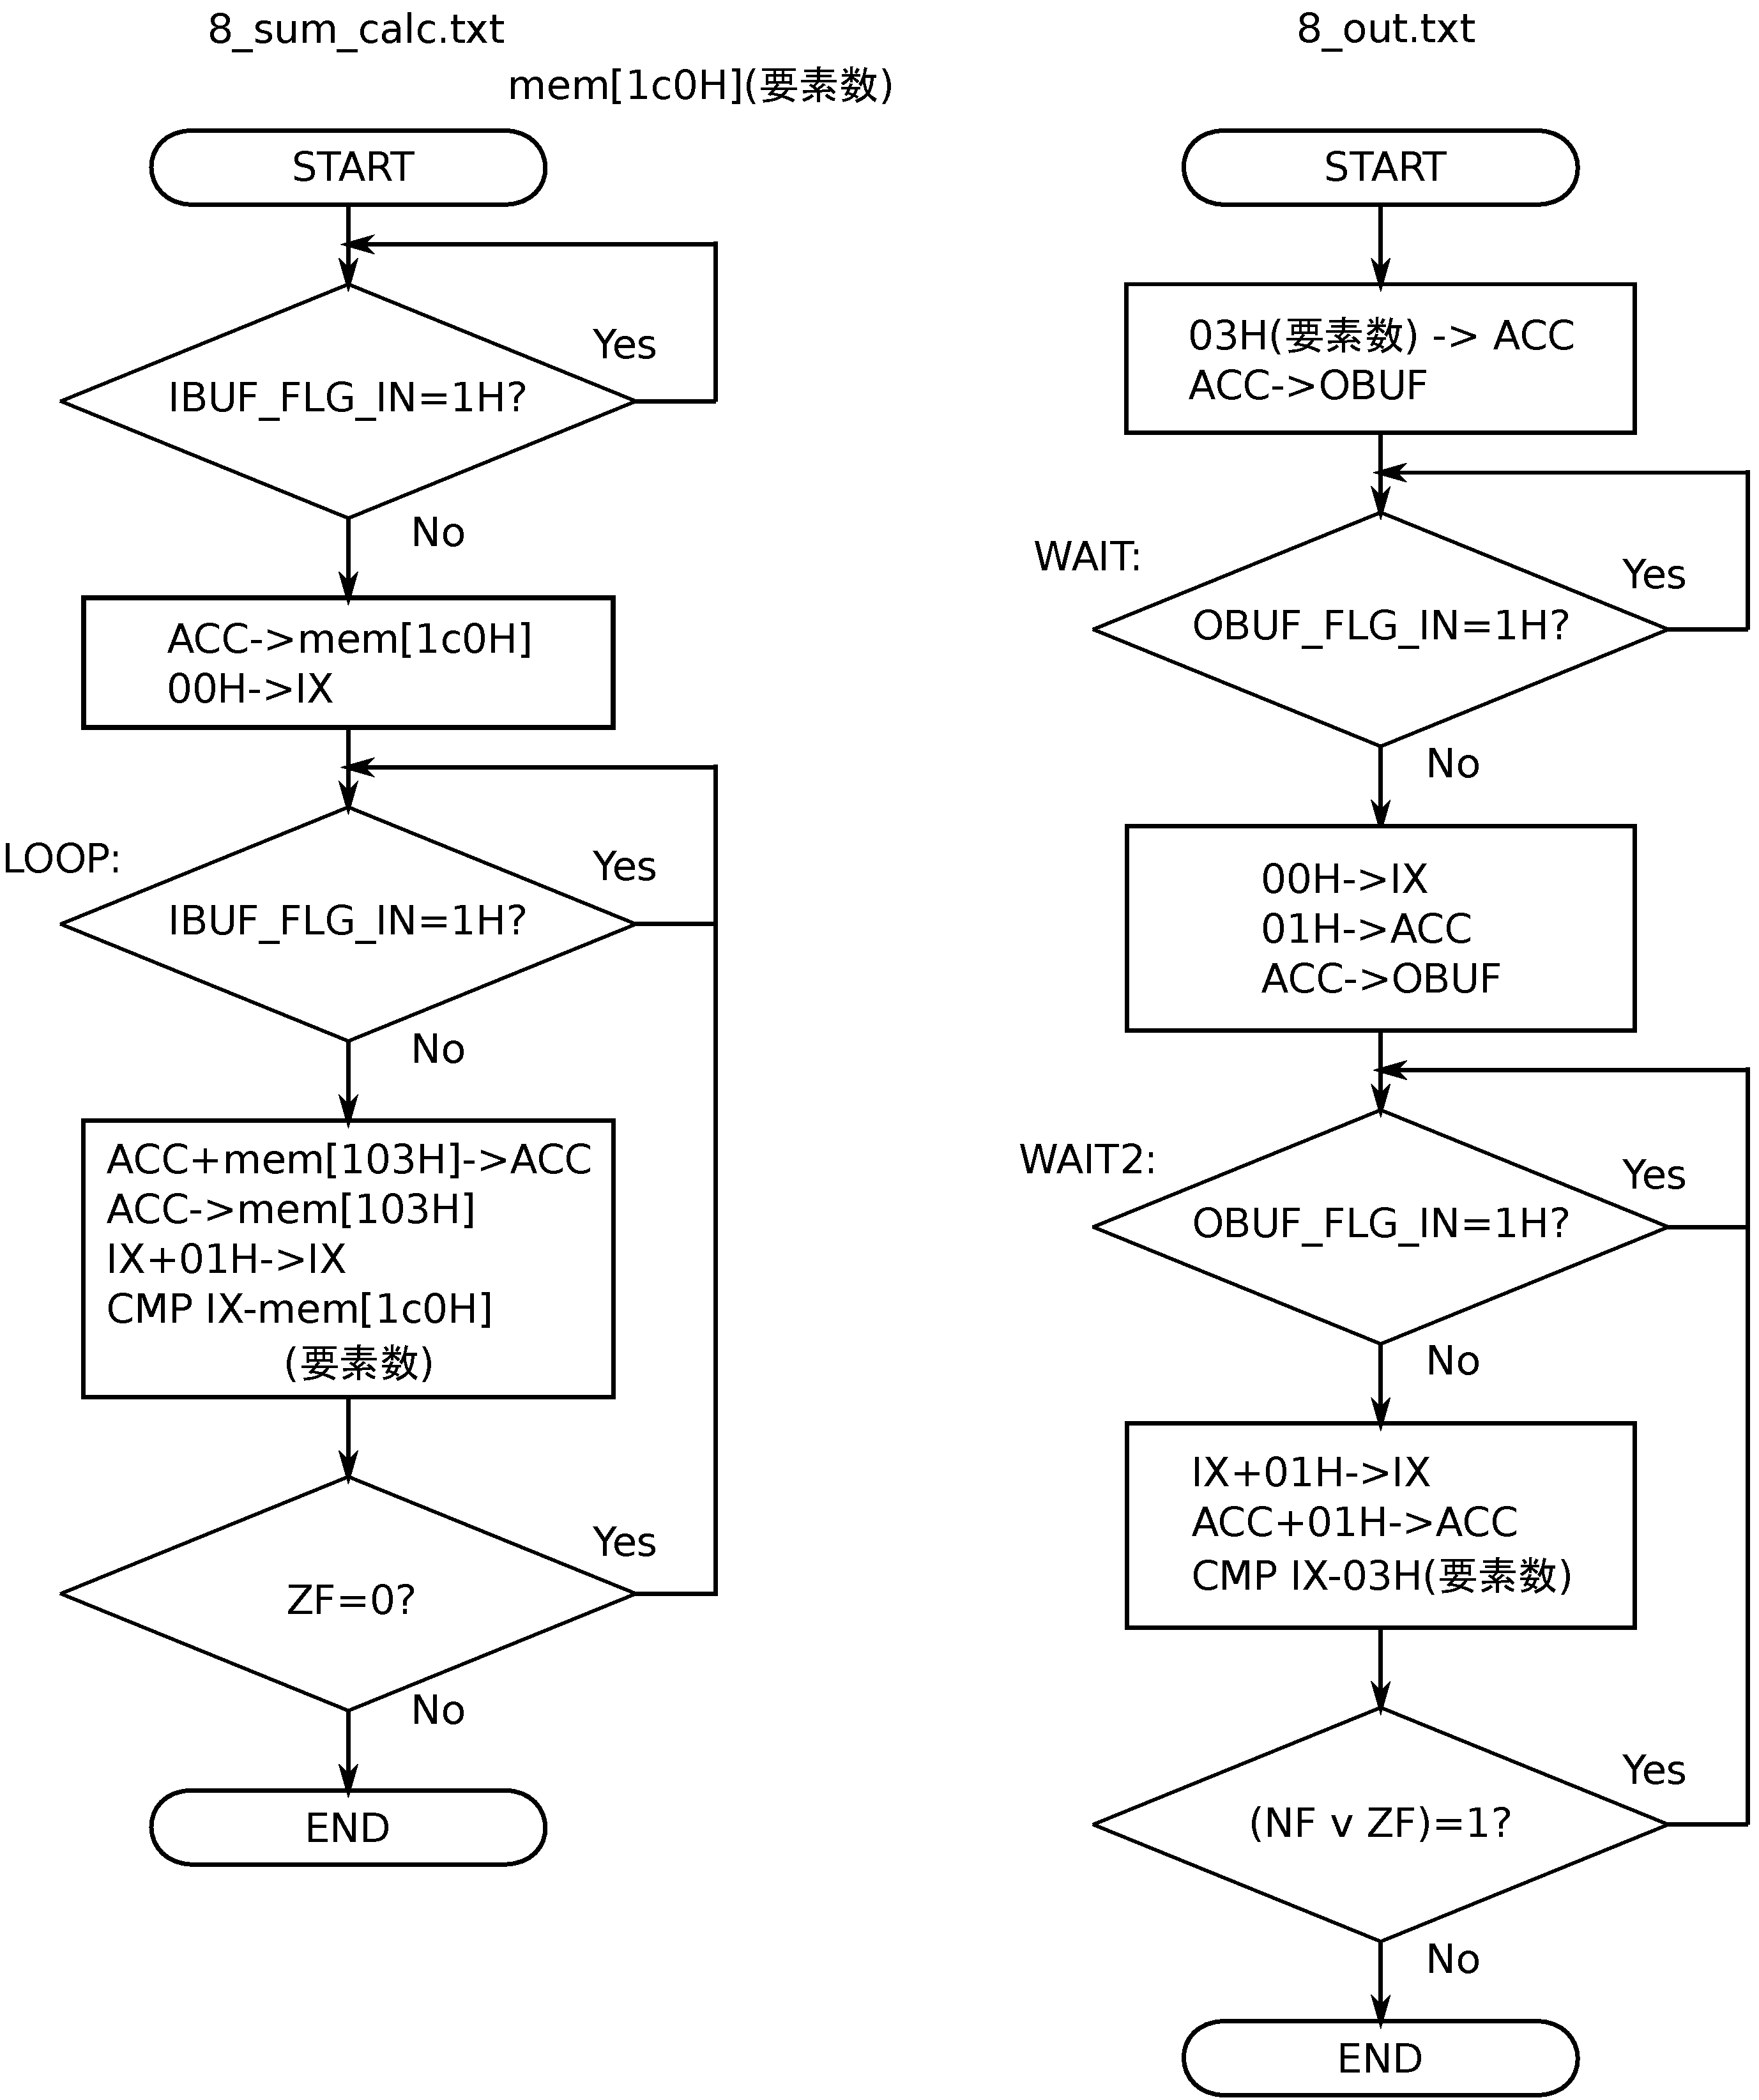
\includegraphics[width=9cm]{8_in_out_flow.pdf}
  \caption{実習8:データ通信プログラムソースコード}
  \label{fig:8_in_out}
\end{figure}

\begin{verbatim}

  CPU0,PC=0x0> r 8_out.txt
  CPU0,PC=0x0> t
  CPU1,PC=0x0> r 8_sum_calc.txt
  CPU1,PC=0x0> i
  CPU1,PC=0x0> i
  CPU1,PC=0x0> t
  CPU0,PC=0x0> i
  CPU0,PC=0x2> i
  CPU0,PC=0x3> t
  CPU1,PC=0x0> i
  CPU1,PC=0x2> d
  	acc=0x00(0,0)    ix=0x00(0,0)   cf=0 vf=0 nf=0 zf=0
  	ibuf=1:0x03(3,3)    obuf=0:0x00(0,0)
  CPU1,PC=0x2> m
      | 000:  34 00 1f 75 c0 6a 00 34    | 008:  07 1f b5 03 75 03 ba 01
      | 010:  fd c0 31 07 0f 00 00 00    | 018:  00 00 00 00 00 00 00 00
      | 020:  00 00 00 00 00 00 00 00    | 028:  00 00 00 00 00 00 00 00
      | 030:  00 00 00 00 00 00 00 00    | 038:  00 00 00 00 00 00 00 00
      | 040:  00 00 00 00 00 00 00 00    | 048:  00 00 00 00 00 00 00 00
      | 050:  00 00 00 00 00 00 00 00    | 058:  00 00 00 00 00 00 00 00
      | 060:  00 00 00 00 00 00 00 00    | 068:  00 00 00 00 00 00 00 00
      | 070:  00 00 00 00 00 00 00 00    | 078:  00 00 00 00 00 00 00 00
      | 080:  00 00 00 00 00 00 00 00    | 088:  00 00 00 00 00 00 00 00
      | 090:  00 00 00 00 00 00 00 00    | 098:  00 00 00 00 00 00 00 00
      | 0a0:  00 00 00 00 00 00 00 00    | 0a8:  00 00 00 00 00 00 00 00
      | 0b0:  00 00 00 00 00 00 00 00    | 0b8:  00 00 00 00 00 00 00 00
      | 0c0:  00 00 00 00 00 00 00 00    | 0c8:  00 00 00 00 00 00 00 00
      | 0d0:  00 00 00 00 00 00 00 00    | 0d8:  00 00 00 00 00 00 00 00
      | 0e0:  00 00 00 00 00 00 00 00    | 0e8:  00 00 00 00 00 00 00 00
      | 0f0:  00 00 00 00 00 00 00 00    | 0f8:  00 00 00 00 00 00 00 00
      | 100:  00 00 00 00 00 00 00 00    | 108:  00 00 00 00 00 00 00 00
      | 110:  00 00 00 00 00 00 00 00    | 118:  00 00 00 00 00 00 00 00
      | 120:  00 00 00 00 00 00 00 00    | 128:  00 00 00 00 00 00 00 00
      | 130:  00 00 00 00 00 00 00 00    | 138:  00 00 00 00 00 00 00 00
      | 140:  00 00 00 00 00 00 00 00    | 148:  00 00 00 00 00 00 00 00
      | 150:  00 00 00 00 00 00 00 00    | 158:  00 00 00 00 00 00 00 00
      | 160:  00 00 00 00 00 00 00 00    | 168:  00 00 00 00 00 00 00 00
      | 170:  00 00 00 00 00 00 00 00    | 178:  00 00 00 00 00 00 00 00
      | 180:  00 00 00 00 00 00 00 00    | 188:  00 00 00 00 00 00 00 00
      | 190:  00 00 00 00 00 00 00 00    | 198:  00 00 00 00 00 00 00 00
      | 1a0:  00 00 00 00 00 00 00 00    | 1a8:  00 00 00 00 00 00 00 00
      | 1b0:  00 00 00 00 00 00 00 00    | 1b8:  00 00 00 00 00 00 00 00
      | 1c0:  00 00 00 00 00 00 00 00    | 1c8:  00 00 00 00 00 00 00 00
      | 1d0:  00 00 00 00 00 00 00 00    | 1d8:  00 00 00 00 00 00 00 00
      | 1e0:  00 00 00 00 00 00 00 00    | 1e8:  00 00 00 00 00 00 00 00
      | 1f0:  00 00 00 00 00 00 00 00    | 1f8:  00 00 00 00 00 00 00 00
  CPU1,PC=0x2> i
  CPU1,PC=0x3> i
  CPU1,PC=0x5> m
      | 000:  34 00 1f 75 c0 6a 00 34    | 008:  07 1f b5 03 75 03 ba 01
      | 010:  fd c0 31 07 0f 00 00 00    | 018:  00 00 00 00 00 00 00 00
      | 020:  00 00 00 00 00 00 00 00    | 028:  00 00 00 00 00 00 00 00
      | 030:  00 00 00 00 00 00 00 00    | 038:  00 00 00 00 00 00 00 00
      | 040:  00 00 00 00 00 00 00 00    | 048:  00 00 00 00 00 00 00 00
      | 050:  00 00 00 00 00 00 00 00    | 058:  00 00 00 00 00 00 00 00
      | 060:  00 00 00 00 00 00 00 00    | 068:  00 00 00 00 00 00 00 00
      | 070:  00 00 00 00 00 00 00 00    | 078:  00 00 00 00 00 00 00 00
      | 080:  00 00 00 00 00 00 00 00    | 088:  00 00 00 00 00 00 00 00
      | 090:  00 00 00 00 00 00 00 00    | 098:  00 00 00 00 00 00 00 00
      | 0a0:  00 00 00 00 00 00 00 00    | 0a8:  00 00 00 00 00 00 00 00
      | 0b0:  00 00 00 00 00 00 00 00    | 0b8:  00 00 00 00 00 00 00 00
      | 0c0:  00 00 00 00 00 00 00 00    | 0c8:  00 00 00 00 00 00 00 00
      | 0d0:  00 00 00 00 00 00 00 00    | 0d8:  00 00 00 00 00 00 00 00
      | 0e0:  00 00 00 00 00 00 00 00    | 0e8:  00 00 00 00 00 00 00 00
      | 0f0:  00 00 00 00 00 00 00 00    | 0f8:  00 00 00 00 00 00 00 00
      | 100:  00 00 00 00 00 00 00 00    | 108:  00 00 00 00 00 00 00 00
      | 110:  00 00 00 00 00 00 00 00    | 118:  00 00 00 00 00 00 00 00
      | 120:  00 00 00 00 00 00 00 00    | 128:  00 00 00 00 00 00 00 00
      | 130:  00 00 00 00 00 00 00 00    | 138:  00 00 00 00 00 00 00 00
      | 140:  00 00 00 00 00 00 00 00    | 148:  00 00 00 00 00 00 00 00
      | 150:  00 00 00 00 00 00 00 00    | 158:  00 00 00 00 00 00 00 00
      | 160:  00 00 00 00 00 00 00 00    | 168:  00 00 00 00 00 00 00 00
      | 170:  00 00 00 00 00 00 00 00    | 178:  00 00 00 00 00 00 00 00
      | 180:  00 00 00 00 00 00 00 00    | 188:  00 00 00 00 00 00 00 00
      | 190:  00 00 00 00 00 00 00 00    | 198:  00 00 00 00 00 00 00 00
      | 1a0:  00 00 00 00 00 00 00 00    | 1a8:  00 00 00 00 00 00 00 00
      | 1b0:  00 00 00 00 00 00 00 00    | 1b8:  00 00 00 00 00 00 00 00
      | 1c0:  03 00 00 00 00 00 00 00    | 1c8:  00 00 00 00 00 00 00 00
      | 1d0:  00 00 00 00 00 00 00 00    | 1d8:  00 00 00 00 00 00 00 00
      | 1e0:  00 00 00 00 00 00 00 00    | 1e8:  00 00 00 00 00 00 00 00
      | 1f0:  00 00 00 00 00 00 00 00    | 1f8:  00 00 00 00 00 00 00 00
  CPU1,PC=0x5> i
  CPU1,PC=0x7> t
  CPU0,PC=0x3> i
  CPU0,PC=0x5> i
  CPU0,PC=0x7> i
  CPU0,PC=0x9> i
  CPU0,PC=0xa> i
  CPU0,PC=0xa> t
  CPU1,PC=0x7> i
  CPU1,PC=0x9> i
  CPU1,PC=0xa> i
  CPU1,PC=0xc> i
  CPU1,PC=0xe> i
  CPU1,PC=0x10> m
      | 000:  34 00 1f 75 c0 6a 00 34    | 008:  07 1f b5 03 75 03 ba 01
      | 010:  fd c0 31 07 0f 00 00 00    | 018:  00 00 00 00 00 00 00 00
      | 020:  00 00 00 00 00 00 00 00    | 028:  00 00 00 00 00 00 00 00
      | 030:  00 00 00 00 00 00 00 00    | 038:  00 00 00 00 00 00 00 00
      | 040:  00 00 00 00 00 00 00 00    | 048:  00 00 00 00 00 00 00 00
      | 050:  00 00 00 00 00 00 00 00    | 058:  00 00 00 00 00 00 00 00
      | 060:  00 00 00 00 00 00 00 00    | 068:  00 00 00 00 00 00 00 00
      | 070:  00 00 00 00 00 00 00 00    | 078:  00 00 00 00 00 00 00 00
      | 080:  00 00 00 00 00 00 00 00    | 088:  00 00 00 00 00 00 00 00
      | 090:  00 00 00 00 00 00 00 00    | 098:  00 00 00 00 00 00 00 00
      | 0a0:  00 00 00 00 00 00 00 00    | 0a8:  00 00 00 00 00 00 00 00
      | 0b0:  00 00 00 00 00 00 00 00    | 0b8:  00 00 00 00 00 00 00 00
      | 0c0:  00 00 00 00 00 00 00 00    | 0c8:  00 00 00 00 00 00 00 00
      | 0d0:  00 00 00 00 00 00 00 00    | 0d8:  00 00 00 00 00 00 00 00
      | 0e0:  00 00 00 00 00 00 00 00    | 0e8:  00 00 00 00 00 00 00 00
      | 0f0:  00 00 00 00 00 00 00 00    | 0f8:  00 00 00 00 00 00 00 00
      | 100:  00 00 00 01 00 00 00 00    | 108:  00 00 00 00 00 00 00 00
      | 110:  00 00 00 00 00 00 00 00    | 118:  00 00 00 00 00 00 00 00
      | 120:  00 00 00 00 00 00 00 00    | 128:  00 00 00 00 00 00 00 00
      | 130:  00 00 00 00 00 00 00 00    | 138:  00 00 00 00 00 00 00 00
      | 140:  00 00 00 00 00 00 00 00    | 148:  00 00 00 00 00 00 00 00
      | 150:  00 00 00 00 00 00 00 00    | 158:  00 00 00 00 00 00 00 00
      | 160:  00 00 00 00 00 00 00 00    | 168:  00 00 00 00 00 00 00 00
      | 170:  00 00 00 00 00 00 00 00    | 178:  00 00 00 00 00 00 00 00
      | 180:  00 00 00 00 00 00 00 00    | 188:  00 00 00 00 00 00 00 00
      | 190:  00 00 00 00 00 00 00 00    | 198:  00 00 00 00 00 00 00 00
      | 1a0:  00 00 00 00 00 00 00 00    | 1a8:  00 00 00 00 00 00 00 00
      | 1b0:  00 00 00 00 00 00 00 00    | 1b8:  00 00 00 00 00 00 00 00
      | 1c0:  03 00 00 00 00 00 00 00    | 1c8:  00 00 00 00 00 00 00 00
      | 1d0:  00 00 00 00 00 00 00 00    | 1d8:  00 00 00 00 00 00 00 00
      | 1e0:  00 00 00 00 00 00 00 00    | 1e8:  00 00 00 00 00 00 00 00
      | 1f0:  00 00 00 00 00 00 00 00    | 1f8:  00 00 00 00 00 00 00 00
  CPU1,PC=0x10> i
  CPU1,PC=0x12> i
  CPU1,PC=0x7> i
  CPU1,PC=0x7> m
      | 000:  34 00 1f 75 c0 6a 00 34    | 008:  07 1f b5 03 75 03 ba 01
      | 010:  fd c0 31 07 0f 00 00 00    | 018:  00 00 00 00 00 00 00 00
      | 020:  00 00 00 00 00 00 00 00    | 028:  00 00 00 00 00 00 00 00
      | 030:  00 00 00 00 00 00 00 00    | 038:  00 00 00 00 00 00 00 00
      | 040:  00 00 00 00 00 00 00 00    | 048:  00 00 00 00 00 00 00 00
      | 050:  00 00 00 00 00 00 00 00    | 058:  00 00 00 00 00 00 00 00
      | 060:  00 00 00 00 00 00 00 00    | 068:  00 00 00 00 00 00 00 00
      | 070:  00 00 00 00 00 00 00 00    | 078:  00 00 00 00 00 00 00 00
      | 080:  00 00 00 00 00 00 00 00    | 088:  00 00 00 00 00 00 00 00
      | 090:  00 00 00 00 00 00 00 00    | 098:  00 00 00 00 00 00 00 00
      | 0a0:  00 00 00 00 00 00 00 00    | 0a8:  00 00 00 00 00 00 00 00
      | 0b0:  00 00 00 00 00 00 00 00    | 0b8:  00 00 00 00 00 00 00 00
      | 0c0:  00 00 00 00 00 00 00 00    | 0c8:  00 00 00 00 00 00 00 00
      | 0d0:  00 00 00 00 00 00 00 00    | 0d8:  00 00 00 00 00 00 00 00
      | 0e0:  00 00 00 00 00 00 00 00    | 0e8:  00 00 00 00 00 00 00 00
      | 0f0:  00 00 00 00 00 00 00 00    | 0f8:  00 00 00 00 00 00 00 00
      | 100:  00 00 00 01 00 00 00 00    | 108:  00 00 00 00 00 00 00 00
      | 110:  00 00 00 00 00 00 00 00    | 118:  00 00 00 00 00 00 00 00
      | 120:  00 00 00 00 00 00 00 00    | 128:  00 00 00 00 00 00 00 00
      | 130:  00 00 00 00 00 00 00 00    | 138:  00 00 00 00 00 00 00 00
      | 140:  00 00 00 00 00 00 00 00    | 148:  00 00 00 00 00 00 00 00
      | 150:  00 00 00 00 00 00 00 00    | 158:  00 00 00 00 00 00 00 00
      | 160:  00 00 00 00 00 00 00 00    | 168:  00 00 00 00 00 00 00 00
      | 170:  00 00 00 00 00 00 00 00    | 178:  00 00 00 00 00 00 00 00
      | 180:  00 00 00 00 00 00 00 00    | 188:  00 00 00 00 00 00 00 00
      | 190:  00 00 00 00 00 00 00 00    | 198:  00 00 00 00 00 00 00 00
      | 1a0:  00 00 00 00 00 00 00 00    | 1a8:  00 00 00 00 00 00 00 00
      | 1b0:  00 00 00 00 00 00 00 00    | 1b8:  00 00 00 00 00 00 00 00
      | 1c0:  03 00 00 00 00 00 00 00    | 1c8:  00 00 00 00 00 00 00 00
      | 1d0:  00 00 00 00 00 00 00 00    | 1d8:  00 00 00 00 00 00 00 00
      | 1e0:  00 00 00 00 00 00 00 00    | 1e8:  00 00 00 00 00 00 00 00
      | 1f0:  00 00 00 00 00 00 00 00    | 1f8:  00 00 00 00 00 00 00 00
  CPU1,PC=0x7> i
  CPU0,PC=0xa> i
  CPU0,PC=0xc> i
  CPU0,PC=0xe> i
  CPU0,PC=0x10> i
  CPU0,PC=0x12> i
  CPU0,PC=0x9> i
  CPU0,PC=0xa> i
  CPU0,PC=0xa> m
      | 000:  62 03 10 3c 03 6a 00 62    | 008:  01 10 3c 0a ba 01 b2 01
      | 010:  fa 03 31 09 0f 00 00 00    | 018:  00 00 00 00 00 00 00 00
      | 020:  00 00 00 00 00 00 00 00    | 028:  00 00 00 00 00 00 00 00
      | 030:  00 00 00 00 00 00 00 00    | 038:  00 00 00 00 00 00 00 00
      | 040:  00 00 00 00 00 00 00 00    | 048:  00 00 00 00 00 00 00 00
      | 050:  00 00 00 00 00 00 00 00    | 058:  00 00 00 00 00 00 00 00
      | 060:  00 00 00 00 00 00 00 00    | 068:  00 00 00 00 00 00 00 00
      | 070:  00 00 00 00 00 00 00 00    | 078:  00 00 00 00 00 00 00 00
      | 080:  00 00 00 00 00 00 00 00    | 088:  00 00 00 00 00 00 00 00
      | 090:  00 00 00 00 00 00 00 00    | 098:  00 00 00 00 00 00 00 00
      | 0a0:  00 00 00 00 00 00 00 00    | 0a8:  00 00 00 00 00 00 00 00
      | 0b0:  00 00 00 00 00 00 00 00    | 0b8:  00 00 00 00 00 00 00 00
      | 0c0:  00 00 00 00 00 00 00 00    | 0c8:  00 00 00 00 00 00 00 00
      | 0d0:  00 00 00 00 00 00 00 00    | 0d8:  00 00 00 00 00 00 00 00
      | 0e0:  00 00 00 00 00 00 00 00    | 0e8:  00 00 00 00 00 00 00 00
      | 0f0:  00 00 00 00 00 00 00 00    | 0f8:  00 00 00 00 00 00 00 00
      | 100:  00 00 00 00 00 00 00 00    | 108:  00 00 00 00 00 00 00 00
      | 110:  00 00 00 00 00 00 00 00    | 118:  00 00 00 00 00 00 00 00
      | 120:  00 00 00 00 00 00 00 00    | 128:  00 00 00 00 00 00 00 00
      | 130:  00 00 00 00 00 00 00 00    | 138:  00 00 00 00 00 00 00 00
      | 140:  00 00 00 00 00 00 00 00    | 148:  00 00 00 00 00 00 00 00
      | 150:  00 00 00 00 00 00 00 00    | 158:  00 00 00 00 00 00 00 00
      | 160:  00 00 00 00 00 00 00 00    | 168:  00 00 00 00 00 00 00 00
      | 170:  00 00 00 00 00 00 00 00    | 178:  00 00 00 00 00 00 00 00
      | 180:  00 00 00 00 00 00 00 00    | 188:  00 00 00 00 00 00 00 00
      | 190:  00 00 00 00 00 00 00 00    | 198:  00 00 00 00 00 00 00 00
      | 1a0:  00 00 00 00 00 00 00 00    | 1a8:  00 00 00 00 00 00 00 00
      | 1b0:  00 00 00 00 00 00 00 00    | 1b8:  00 00 00 00 00 00 00 00
      | 1c0:  00 00 00 00 00 00 00 00    | 1c8:  00 00 00 00 00 00 00 00
      | 1d0:  00 00 00 00 00 00 00 00    | 1d8:  00 00 00 00 00 00 00 00
      | 1e0:  00 00 00 00 00 00 00 00    | 1e8:  00 00 00 00 00 00 00 00
      | 1f0:  00 00 00 00 00 00 00 00    | 1f8:  00 00 00 00 00 00 00 00
  CPU0,PC=0xa> i
  CPU1,PC=0x7> i
  CPU1,PC=0x9> i
  CPU1,PC=0xa> i
  CPU1,PC=0xc> m
      | 000:  34 00 1f 75 c0 6a 00 34    | 008:  07 1f b5 03 75 03 ba 01
      | 010:  fd c0 31 07 0f 00 00 00    | 018:  00 00 00 00 00 00 00 00
      | 020:  00 00 00 00 00 00 00 00    | 028:  00 00 00 00 00 00 00 00
      | 030:  00 00 00 00 00 00 00 00    | 038:  00 00 00 00 00 00 00 00
      | 040:  00 00 00 00 00 00 00 00    | 048:  00 00 00 00 00 00 00 00
      | 050:  00 00 00 00 00 00 00 00    | 058:  00 00 00 00 00 00 00 00
      | 060:  00 00 00 00 00 00 00 00    | 068:  00 00 00 00 00 00 00 00
      | 070:  00 00 00 00 00 00 00 00    | 078:  00 00 00 00 00 00 00 00
      | 080:  00 00 00 00 00 00 00 00    | 088:  00 00 00 00 00 00 00 00
      | 090:  00 00 00 00 00 00 00 00    | 098:  00 00 00 00 00 00 00 00
      | 0a0:  00 00 00 00 00 00 00 00    | 0a8:  00 00 00 00 00 00 00 00
      | 0b0:  00 00 00 00 00 00 00 00    | 0b8:  00 00 00 00 00 00 00 00
      | 0c0:  00 00 00 00 00 00 00 00    | 0c8:  00 00 00 00 00 00 00 00
      | 0d0:  00 00 00 00 00 00 00 00    | 0d8:  00 00 00 00 00 00 00 00
      | 0e0:  00 00 00 00 00 00 00 00    | 0e8:  00 00 00 00 00 00 00 00
      | 0f0:  00 00 00 00 00 00 00 00    | 0f8:  00 00 00 00 00 00 00 00
      | 100:  00 00 00 01 00 00 00 00    | 108:  00 00 00 00 00 00 00 00
      | 110:  00 00 00 00 00 00 00 00    | 118:  00 00 00 00 00 00 00 00
      | 120:  00 00 00 00 00 00 00 00    | 128:  00 00 00 00 00 00 00 00
      | 130:  00 00 00 00 00 00 00 00    | 138:  00 00 00 00 00 00 00 00
      | 140:  00 00 00 00 00 00 00 00    | 148:  00 00 00 00 00 00 00 00
      | 150:  00 00 00 00 00 00 00 00    | 158:  00 00 00 00 00 00 00 00
      | 160:  00 00 00 00 00 00 00 00    | 168:  00 00 00 00 00 00 00 00
      | 170:  00 00 00 00 00 00 00 00    | 178:  00 00 00 00 00 00 00 00
      | 180:  00 00 00 00 00 00 00 00    | 188:  00 00 00 00 00 00 00 00
      | 190:  00 00 00 00 00 00 00 00    | 198:  00 00 00 00 00 00 00 00
      | 1a0:  00 00 00 00 00 00 00 00    | 1a8:  00 00 00 00 00 00 00 00
      | 1b0:  00 00 00 00 00 00 00 00    | 1b8:  00 00 00 00 00 00 00 00
      | 1c0:  03 00 00 00 00 00 00 00    | 1c8:  00 00 00 00 00 00 00 00
      | 1d0:  00 00 00 00 00 00 00 00    | 1d8:  00 00 00 00 00 00 00 00
      | 1e0:  00 00 00 00 00 00 00 00    | 1e8:  00 00 00 00 00 00 00 00
      | 1f0:  00 00 00 00 00 00 00 00    | 1f8:  00 00 00 00 00 00 00 00
  CPU1,PC=0xc> i
  CPU1,PC=0xe> i
  CPU1,PC=0x10> i
  CPU1,PC=0x12> i
  CPU1,PC=0x7> i
  CPU1,PC=0x7> m
      | 000:  34 00 1f 75 c0 6a 00 34    | 008:  07 1f b5 03 75 03 ba 01
      | 010:  fd c0 31 07 0f 00 00 00    | 018:  00 00 00 00 00 00 00 00
      | 020:  00 00 00 00 00 00 00 00    | 028:  00 00 00 00 00 00 00 00
      | 030:  00 00 00 00 00 00 00 00    | 038:  00 00 00 00 00 00 00 00
      | 040:  00 00 00 00 00 00 00 00    | 048:  00 00 00 00 00 00 00 00
      | 050:  00 00 00 00 00 00 00 00    | 058:  00 00 00 00 00 00 00 00
      | 060:  00 00 00 00 00 00 00 00    | 068:  00 00 00 00 00 00 00 00
      | 070:  00 00 00 00 00 00 00 00    | 078:  00 00 00 00 00 00 00 00
      | 080:  00 00 00 00 00 00 00 00    | 088:  00 00 00 00 00 00 00 00
      | 090:  00 00 00 00 00 00 00 00    | 098:  00 00 00 00 00 00 00 00
      | 0a0:  00 00 00 00 00 00 00 00    | 0a8:  00 00 00 00 00 00 00 00
      | 0b0:  00 00 00 00 00 00 00 00    | 0b8:  00 00 00 00 00 00 00 00
      | 0c0:  00 00 00 00 00 00 00 00    | 0c8:  00 00 00 00 00 00 00 00
      | 0d0:  00 00 00 00 00 00 00 00    | 0d8:  00 00 00 00 00 00 00 00
      | 0e0:  00 00 00 00 00 00 00 00    | 0e8:  00 00 00 00 00 00 00 00
      | 0f0:  00 00 00 00 00 00 00 00    | 0f8:  00 00 00 00 00 00 00 00
      | 100:  00 00 00 03 00 00 00 00    | 108:  00 00 00 00 00 00 00 00
      | 110:  00 00 00 00 00 00 00 00    | 118:  00 00 00 00 00 00 00 00
      | 120:  00 00 00 00 00 00 00 00    | 128:  00 00 00 00 00 00 00 00
      | 130:  00 00 00 00 00 00 00 00    | 138:  00 00 00 00 00 00 00 00
      | 140:  00 00 00 00 00 00 00 00    | 148:  00 00 00 00 00 00 00 00
      | 150:  00 00 00 00 00 00 00 00    | 158:  00 00 00 00 00 00 00 00
      | 160:  00 00 00 00 00 00 00 00    | 168:  00 00 00 00 00 00 00 00
      | 170:  00 00 00 00 00 00 00 00    | 178:  00 00 00 00 00 00 00 00
      | 180:  00 00 00 00 00 00 00 00    | 188:  00 00 00 00 00 00 00 00
      | 190:  00 00 00 00 00 00 00 00    | 198:  00 00 00 00 00 00 00 00
      | 1a0:  00 00 00 00 00 00 00 00    | 1a8:  00 00 00 00 00 00 00 00
      | 1b0:  00 00 00 00 00 00 00 00    | 1b8:  00 00 00 00 00 00 00 00
      | 1c0:  03 00 00 00 00 00 00 00    | 1c8:  00 00 00 00 00 00 00 00
      | 1d0:  00 00 00 00 00 00 00 00    | 1d8:  00 00 00 00 00 00 00 00
      | 1e0:  00 00 00 00 00 00 00 00    | 1e8:  00 00 00 00 00 00 00 00
      | 1f0:  00 00 00 00 00 00 00 00    | 1f8:  00 00 00 00 00 00 00 00
  CPU1,PC=0x7> t
  CPU0,PC=0xa> i
  CPU0,PC=0xc> i
  CPU0,PC=0xe> i
  CPU0,PC=0x10> i
  CPU0,PC=0x12> i
  CPU0,PC=0x9> i
  CPU0,PC=0xa> i
  CPU0,PC=0xa> t
  CPU1,PC=0x7> t
  CPU0,PC=0xa> m
      | 000:  62 03 10 3c 03 6a 00 62    | 008:  01 10 3c 0a ba 01 b2 01
      | 010:  fa 03 31 09 0f 00 00 00    | 018:  00 00 00 00 00 00 00 00
      | 020:  00 00 00 00 00 00 00 00    | 028:  00 00 00 00 00 00 00 00
      | 030:  00 00 00 00 00 00 00 00    | 038:  00 00 00 00 00 00 00 00
      | 040:  00 00 00 00 00 00 00 00    | 048:  00 00 00 00 00 00 00 00
      | 050:  00 00 00 00 00 00 00 00    | 058:  00 00 00 00 00 00 00 00
      | 060:  00 00 00 00 00 00 00 00    | 068:  00 00 00 00 00 00 00 00
      | 070:  00 00 00 00 00 00 00 00    | 078:  00 00 00 00 00 00 00 00
      | 080:  00 00 00 00 00 00 00 00    | 088:  00 00 00 00 00 00 00 00
      | 090:  00 00 00 00 00 00 00 00    | 098:  00 00 00 00 00 00 00 00
      | 0a0:  00 00 00 00 00 00 00 00    | 0a8:  00 00 00 00 00 00 00 00
      | 0b0:  00 00 00 00 00 00 00 00    | 0b8:  00 00 00 00 00 00 00 00
      | 0c0:  00 00 00 00 00 00 00 00    | 0c8:  00 00 00 00 00 00 00 00
      | 0d0:  00 00 00 00 00 00 00 00    | 0d8:  00 00 00 00 00 00 00 00
      | 0e0:  00 00 00 00 00 00 00 00    | 0e8:  00 00 00 00 00 00 00 00
      | 0f0:  00 00 00 00 00 00 00 00    | 0f8:  00 00 00 00 00 00 00 00
      | 100:  00 00 00 00 00 00 00 00    | 108:  00 00 00 00 00 00 00 00
      | 110:  00 00 00 00 00 00 00 00    | 118:  00 00 00 00 00 00 00 00
      | 120:  00 00 00 00 00 00 00 00    | 128:  00 00 00 00 00 00 00 00
      | 130:  00 00 00 00 00 00 00 00    | 138:  00 00 00 00 00 00 00 00
      | 140:  00 00 00 00 00 00 00 00    | 148:  00 00 00 00 00 00 00 00
      | 150:  00 00 00 00 00 00 00 00    | 158:  00 00 00 00 00 00 00 00
      | 160:  00 00 00 00 00 00 00 00    | 168:  00 00 00 00 00 00 00 00
      | 170:  00 00 00 00 00 00 00 00    | 178:  00 00 00 00 00 00 00 00
      | 180:  00 00 00 00 00 00 00 00    | 188:  00 00 00 00 00 00 00 00
      | 190:  00 00 00 00 00 00 00 00    | 198:  00 00 00 00 00 00 00 00
      | 1a0:  00 00 00 00 00 00 00 00    | 1a8:  00 00 00 00 00 00 00 00
      | 1b0:  00 00 00 00 00 00 00 00    | 1b8:  00 00 00 00 00 00 00 00
      | 1c0:  00 00 00 00 00 00 00 00    | 1c8:  00 00 00 00 00 00 00 00
      | 1d0:  00 00 00 00 00 00 00 00    | 1d8:  00 00 00 00 00 00 00 00
      | 1e0:  00 00 00 00 00 00 00 00    | 1e8:  00 00 00 00 00 00 00 00
      | 1f0:  00 00 00 00 00 00 00 00    | 1f8:  00 00 00 00 00 00 00 00
  CPU0,PC=0xa> t
  CPU1,PC=0x7> i
  CPU1,PC=0x9> i
  CPU1,PC=0xa> i
  CPU1,PC=0xc> i
  CPU1,PC=0xe> i
  CPU1,PC=0x10> i
  CPU1,PC=0x12> i
  CPU1,PC=0x14> i
  Program Halted.
  CPU1,PC=0x15> m
      | 000:  34 00 1f 75 c0 6a 00 34    | 008:  07 1f b5 03 75 03 ba 01
      | 010:  fd c0 31 07 0f 00 00 00    | 018:  00 00 00 00 00 00 00 00
      | 020:  00 00 00 00 00 00 00 00    | 028:  00 00 00 00 00 00 00 00
      | 030:  00 00 00 00 00 00 00 00    | 038:  00 00 00 00 00 00 00 00
      | 040:  00 00 00 00 00 00 00 00    | 048:  00 00 00 00 00 00 00 00
      | 050:  00 00 00 00 00 00 00 00    | 058:  00 00 00 00 00 00 00 00
      | 060:  00 00 00 00 00 00 00 00    | 068:  00 00 00 00 00 00 00 00
      | 070:  00 00 00 00 00 00 00 00    | 078:  00 00 00 00 00 00 00 00
      | 080:  00 00 00 00 00 00 00 00    | 088:  00 00 00 00 00 00 00 00
      | 090:  00 00 00 00 00 00 00 00    | 098:  00 00 00 00 00 00 00 00
      | 0a0:  00 00 00 00 00 00 00 00    | 0a8:  00 00 00 00 00 00 00 00
      | 0b0:  00 00 00 00 00 00 00 00    | 0b8:  00 00 00 00 00 00 00 00
      | 0c0:  00 00 00 00 00 00 00 00    | 0c8:  00 00 00 00 00 00 00 00
      | 0d0:  00 00 00 00 00 00 00 00    | 0d8:  00 00 00 00 00 00 00 00
      | 0e0:  00 00 00 00 00 00 00 00    | 0e8:  00 00 00 00 00 00 00 00
      | 0f0:  00 00 00 00 00 00 00 00    | 0f8:  00 00 00 00 00 00 00 00
      | 100:  00 00 00 06 00 00 00 00    | 108:  00 00 00 00 00 00 00 00
      | 110:  00 00 00 00 00 00 00 00    | 118:  00 00 00 00 00 00 00 00
      | 120:  00 00 00 00 00 00 00 00    | 128:  00 00 00 00 00 00 00 00
      | 130:  00 00 00 00 00 00 00 00    | 138:  00 00 00 00 00 00 00 00
      | 140:  00 00 00 00 00 00 00 00    | 148:  00 00 00 00 00 00 00 00
      | 150:  00 00 00 00 00 00 00 00    | 158:  00 00 00 00 00 00 00 00
      | 160:  00 00 00 00 00 00 00 00    | 168:  00 00 00 00 00 00 00 00
      | 170:  00 00 00 00 00 00 00 00    | 178:  00 00 00 00 00 00 00 00
      | 180:  00 00 00 00 00 00 00 00    | 188:  00 00 00 00 00 00 00 00
      | 190:  00 00 00 00 00 00 00 00    | 198:  00 00 00 00 00 00 00 00
      | 1a0:  00 00 00 00 00 00 00 00    | 1a8:  00 00 00 00 00 00 00 00
      | 1b0:  00 00 00 00 00 00 00 00    | 1b8:  00 00 00 00 00 00 00 00
      | 1c0:  03 00 00 00 00 00 00 00    | 1c8:  00 00 00 00 00 00 00 00
      | 1d0:  00 00 00 00 00 00 00 00    | 1d8:  00 00 00 00 00 00 00 00
      | 1e0:  00 00 00 00 00 00 00 00    | 1e8:  00 00 00 00 00 00 00 00
      | 1f0:  00 00 00 00 00 00 00 00    | 1f8:  00 00 00 00 00 00 00 00
  CPU1,PC=0x15> 


\end{verbatim}
\newpage

\section{演習}
  \subsection{演習4}
  教育用CPUボードでもJR,JAL命令を用いなくてもサブルーチンを実現することは可能だと考える.理由としては関数に飛ぶ際にフラグ用のメモリを用意し関数(サブルーチン)を用いる際は1にして条件 Branch命令を用いて関数の動作内容が記述されている部分にPCを変更する.事前に戻る位置のPCはどこかのメモリに記録しておき,戻る前にフラグ用のメモリを0へ戻してBranch命令を用い戻るいちを記録したメモリを参照しPCを変更させることにより実現できると考えた.
\section{考察}
cpuシミュレータ作成実習を通して,各マシン命令を作成することによってフェーズ毎の動作を知ることができた.メモリを意識しながらプログラムを行うことによってC言語のポインタに対する考えが深まった.普段pythonやc言語などを用いるためマシン語でコーディングする際に理解しにくくミスが増えプログラミングの効率が悪く時間も多くかかってしまった,現在利用されている言語は人間が用いる言葉に近い形で記述することができより良い形に使用される言語も変化しているのだと感じられた.
                                                                               %鉋 謹製ソフトが便利かもhttps://github.com/TateIsuKanna/TeXreferenceURL
    \begin{thebibliography}{9}
      %  \bibitem{cabbage}野菜類/(キャベツ類)/キャベツ/結球葉,生 \url{https://fooddb.mext.go.jp/details/details.pl?ITEM_NO=06_06061_6} 2018/10/18閲覧
        \bibitem{sidousyo}CPU実習テキスト
        \bibitem{cpu_use_book}教育用CPUボードのマニュアル
  %      \bibitem{lettuce}野菜類/(レタス類)/レタス/土耕栽培/結球葉/生 \url{https://fooddb.mext.go.jp/details/details.pl?ITEM_NO=06_06312_6} 2018/10/18閲覧
    \end{thebibliography}
\end{document}
